% Standalone source for figures/solution-flowchart.png (JOSS paper).
% Build:  pdflatex solution-flowchart
%         pdftocairo -png -r 300 -singlefile solution-flowchart.pdf solution-flowchart
\documentclass[tikz,border=2mm]{standalone}
\usetikzlibrary{arrows.meta,positioning,shapes.geometric}

\begin{document}
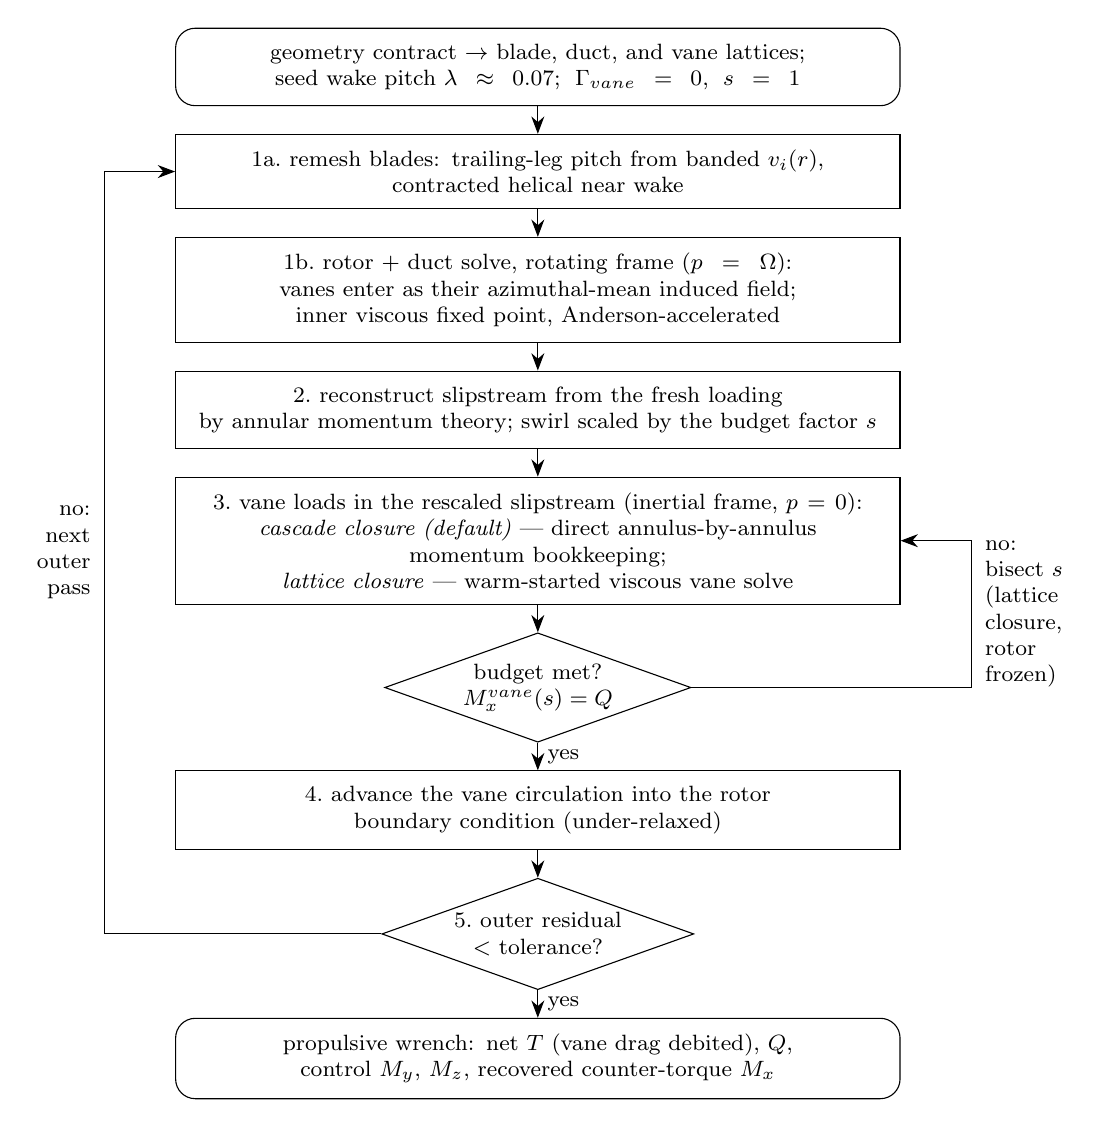
\begin{tikzpicture}[
  font=\footnotesize,
  node distance=3.5mm,
  term/.style={draw, rounded corners=2.5mm, align=center,
               inner sep=2mm, text width=88mm},
  proc/.style={draw, align=center, inner sep=2mm, text width=88mm},
  dec/.style={draw, diamond, aspect=2.8, align=center, inner sep=0.4mm},
  arr/.style={-{Stealth[length=2.2mm]}}
]
  \node[term] (start) {geometry contract $\to$ blade, duct, and vane
    lattices;\\ seed wake pitch $\lambda \approx 0.07$;\;
    $\Gamma_{vane} = 0$,\; $s = 1$};
  \node[proc, below=of start] (remesh) {1a.\ remesh blades:
    trailing-leg pitch from banded $v_i(r)$,\\
    contracted helical near wake};
  \node[proc, below=of remesh] (rotor) {1b.\ rotor $+$ duct solve,
    rotating frame ($p = \Omega$):\\
    vanes enter as their azimuthal-mean induced field;\\
    inner viscous fixed point, Anderson-accelerated};
  \node[proc, below=of rotor] (slip) {2.\ reconstruct slipstream from
    the fresh loading\\ by annular momentum theory; swirl scaled by
    the budget factor $s$};
  \node[proc, below=of slip] (vane) {3.\ vane loads in the rescaled
    slipstream (inertial frame, $p = 0$):\\
    \emph{cascade closure (default)} --- direct annulus-by-annulus\\
    momentum bookkeeping;\\
    \emph{lattice closure} --- warm-started viscous vane solve};
  \node[dec, below=of vane] (bud) {budget met?\\
    $M_x^{vane}(s) = Q$};
  \node[proc, below=of bud] (fb) {4.\ advance the vane circulation
    into the rotor\\ boundary condition (under-relaxed)};
  \node[dec, below=of fb] (conv) {5.\ outer residual\\
    $<$ tolerance?};
  \node[term, below=of conv] (out) {propulsive wrench: net $T$ (vane
    drag debited), $Q$,\\ control $M_y$, $M_z$, recovered
    counter-torque $M_x$};

  \draw[arr] (start) -- (remesh);
  \draw[arr] (remesh) -- (rotor);
  \draw[arr] (rotor) -- (slip);
  \draw[arr] (slip) -- (vane);
  \draw[arr] (vane) -- (bud);
  \draw[arr] (bud) -- node[right]{yes} (fb);
  \draw[arr] (fb) -- (conv);
  \draw[arr] (conv) -- node[right]{yes} (out);
  \draw[arr] (bud.east) -|
    node[pos=0.75, right=0.5mm, align=left]{no:\\ bisect $s$\\ (lattice\\ closure,\\ rotor\\ frozen)}
    ([xshift=9mm]vane.east) -- (vane.east);
  \draw[arr] (conv.west) -|
    node[pos=0.75, left=0.5mm, align=right]{no:\\ next\\ outer\\ pass}
    ([xshift=-9mm]remesh.west) -- (remesh.west);
\end{tikzpicture}
\end{document}
